\subsection{Multi-authority attribute based encryption}
In this section the field of Multi-authority attribute-based encryption (\ac{MA-ABE}) will be evaluated more deeply with respect to all requirements of section \ref{sec:requierements}. 

Another notable technique recently used by \cite{yang2013dac}, \cite{wu2017security}, \cite{li2017two} and \cite{wang2011hierarchical} is \textit{proxy de-/reencryption}. It is motivated by the fact that mobile devices often don't have much computing resources so that the server may help the clients for decryption. The main idea is that the server does the preprocessing of the encrypted text given paramteres by the user. In the end the preprocessed encrypted content will be easily computable by the edge device. The cural fact is that the server will have no knowledge about the plaintext but rather helps the user on decryption or reencryption. 

In the following the different sub topics of \ac{MA-ABE} will be described, analyzed given the requirement set and finally evaluated based on their perforamnce and scalability. 

\subsubsection{Introduction into Multi-Authority Attribute-based Encryption}
Chase 2007 \cite{chase2007multi} was the frist known to introduce the first \ac{MA-ABE} schemes. In her paper she describes the process on how to derrive a multi-authority attribute-based encryption scheme vom the single authrotity schemes. 

The collussion resistance criteria in \ac{ABE} implies that any data owner needs to encrypt under attributes in such kind that the ciphertext is independent of any users specific identifiers. Any user could in theory decrypter the ciphertext if he holds the fullfilling attribute set. While chase's scheme also used bilinear maps it main security was based on interpolation and the fact that no underdefined linaer equation system could definitly be solved\footnote{For \ac{LSSS} matrix are based on the same assumption.}.  

Colluding users can not decrypter any cipher text and the plain text is encrypted using a blinded master secret. The blinding factor is then implemented in the policy so that any user satisfying this policy can restore the blinding factor and so revocer the plaintext. 

In the next step each user is given blinded attribute private keys so that when used on decryption the plaintext is still blinded with the user specific identifier. Using pairings this identifier can be substituted and the plaintext gets revealed. 

Two cural disadventages where not respected by chase in her initial scheme. First the \ac{CA} had global decryption power. It needed to issue each \ac{AA} a specific seed so that on using this seed in a pheudo random generator the \ac{CA} knew what random value would be calculated. This was importent since the \ac{CA} need to isse the user his private key which combined with the private attribute keys from the \ac{AA} would reveal on decryption the unblinded plaintext. 

Chase improved her scheme 2009 in \cite{chase2009improving}. Now all \ac{AA}s will do a n-party key exchange to distribute the secret seeds with each other. Agreeing on a well known value the \ac{CA} was no longer needed and as long $N-2$ \ac{AA}s are not colluding with each other the secret remained secure. 

The other disadventage, that was will present in the updated scheme, was that no new \ac{AA} could be added after system inizialisation since it would trigger a new system inizialisation and distribution of the master secret. 

The lack of addition new attribute authorities and the missing revocation scheme made chases scheme impractical for further evaluations but give a good introduction the fitfalls of \ac{MA-ABE} schemes.

\subsubsection{Hirachical \ac{ABE}}
\label{sec:HABE}

\begin{figure*}[!ht]
\centering
    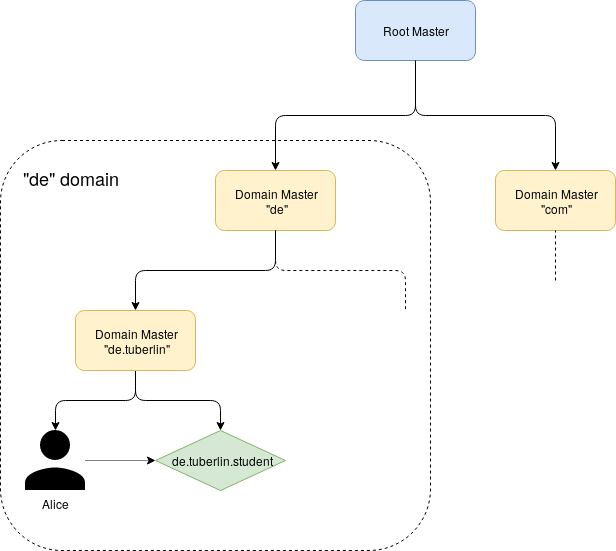
\includegraphics[width=0.5\linewidth]{img/HABE.png}
    \caption{Structe of hirachical attribute-based encryption systems}
    \label{fig:habe}
\end{figure*}

Hirachical Attribute-Based encryption (\ac{HABE}) takes the key delegation one step further. It is sourly designed arround the idea that if a private key exist that have a certain access power, it is possible for the key holder to deletate a subset of his access power to a new instance. By nature follows a hirachical structure where each user could administrate an own subdomain. Here many use cases for cloud computing as well as cloud storage system emerged. \cite{Wang:2010:HAE:1866307.1866414}. While some works also take revocation into design a cural requirement is still missing.

As displayed in figure \ref{fig:habe}, which is based on the approach in \cite{wang2011hierarchical}, the root master summarized the global decryption power of the system and can set up new domain masters (attribute authorities). They on the other hand can delegate a subset of decryption power to a sub domain master. Each domain master can administer users and attributes.

Hirachical \ac{ABE} is the predecessor of Multi-Authority Attribute based encryption. The differences can be summarized by the following points: In \ac{MA-ABE} each user is assigned to a specific attribute authority. This must not be the case in \ac{HABE}. \ac{HABE} is tree-like orientated. Starting from the root node each following authority will have a subset of decryption power as its respectiv parent. 

\cite{Wang:2010:HAE:1866307.1866414} formalized this approach using \ac{CP-ABE}, which was later extended in \cite{wang2011hierarchical}. While implementing a revocation scheme, they depend on an access policy present in \ac{DNF}, which might not always be possible without using negation. 

A hirachical strcture and a delegation of decryption power would, as already mentioned, imply that the root master has global decryption power which is not desired \req{C4}. We want to design a system in which each domain is seperated is term of key generation from each other. That means that there is no top level domain which has global decryption power, rather we want to have a system where each subdomain creates its down keys and administrataes thier own attributes but that is still a part of a bigger system so able to interact with other domains.  
\todo{Reformulate}

\subsubsection{Decentralized attribute-based encryption}
\label{sec:DABE}
Both issues where addressed with the sub topic of \textit{decentralized attribute based encryption} (\ac{DABE}). As the name indicates \ac{DABE} does not need a \ac{CA} managing the setup of additional \ac{AA}s. This ecosystem is self sustaining in the form that each entity can become an \ac{AA} if needed and start issuing new attributes to users. 

Some form of centralization must be still preserved. The global paramter for example needs to be known to each new entity and each user usally need to get a unique global identifier to be identified among the set of users. Also attributes need to be somehow syncronized since the set of attriubte identifier usally need to be non intersecting across different domains. All this information could be published by a public bullitin board and was first proposed by \cite{lewko2011decentralizing}. 

Revocation in such system remains an open issue. Since no central authority manages all users, no authority can be in charge of revocing them. An authroity could revoce its issued attributes but only in an indirct fassion since decentralzied systems are build around the idea that nodes can go offline at any time. If an authority would go offline as soon at it received the revocation request the revocation procedure would never trigger. 

Cui and Deng showed in \cite{cui2016revocable} that such a system could exist. Each key and ciphertext got a liveness assigned that is active for a certain time periode. After the time periode expired all keys need to be reissed by each \ac{AA}. Indirect revocation happens by simply not reissuing a user certain attribute keys. This sytem is implemented in the comparison in \ref{sec:ma-comparison}.

The question remains if such a system would be practically applicable since each cipher text needs to be reuploaded in each time periode. Revocation in decentralized attribute based encryption remains an open issue.

\subsubsection{Efficient Data Access Control for Multi-Authority Cloud Storage}
The most explored field in \ac{MA-ABE} is the Efficient Data Access Control for Multi-Authrotity Cloud Stroage (\ac{DAC-MACS}) family \cite{yang2013dac}. First instroducted by Yang \textit{et. al.} 2013 it desribes an efficient, revocable \ac{MA-ABE} scheme based on \ac{CP-ABE} and using proxy encryption on decryption and reencryption. Furhter this scheme features a large attribute universe, adding \ac{AA}s on the running system and serves with a \ac{CA} that has no global decryption power. In sort \ac{DAC-MACS} satisfy all the non-optional requirements.

\ac{DAC-MACS} elliminates the need for the global decryption power of the \ac{CA} by issuing $k$ ciphertexts: One per \ac{AA}. \footnote{If the ciphertext does not require any attributes of an specific authority it does not have to create a ciphertext for this domain.} It does not require any coordination between authorities which enables to add new \ac{AA}s at runtime without recreating the user keys. This scheme also includes features for efficient revocation while it claims to maintain forward and backward secrecy.

\ac{DAC-MACS} is not collusion resistance on attribute revocation under the active attack model. The scheme \ac{NEDAC-MACS} (New Extended \ac{DAC-MACS}) shows and solves this vulnerability \cite{wu2017security}. Recent studies introduce a more efficient, scalable and secure approaches such as \ac{MAACS} \cite{li2016secure} and \ac{TF-DAC-MACS} (Two-Factor \ac{DAC-MACS})\cite{li2017two}. 

All the \ac{DAC-MACS} schemes are structed in roughly the same way. They usally describe six different entities:

\begin{enumerate}
	\item \textbf{Certificate/Central Authority (\ac{CA})} The purpose of the \ac{CA} is to issue user their global identifier (\ac{GID}). Furhter they bootstrap the different \ac{AA}s. The \ac{CA} remains trusted but do not have any decryption power in the system. 
	\item \textbf{Attribute Authority (\ac{AA})} A attribute authority administers their domain. Issues attributes and their respective privat key to the user. They only accept a user if his \ac{GID} is signed by the \ac{CA}. 
	On revocation they will need to update the users secret keys as well as the ciphertext encrypted with the revoked attribute key. \ac{AA}s are assumed to be trusted but can be compromised by an adversary.
	\item \textbf{Server} The purpose of the server is to help the user with proxy re- and decryption. If an \ac{AA} broadcast a revocation of an attribute, the server may download all related ciphertexts from the \ac{CSP} to update them with the new attribute. 
	Further, the user may give the server his attribute privat keys so that the server can pre compute the ciphertext. Usally the thread model for the server is honest-but-curious. Please note, that the \ac{CA} and the server are two seperated entities that do not cooperate.
	\item \textbf{Data owner} The data owner are usally users who want to encrypt content with under a specific access policy. To do so they use the publically available public keys pinned on the public bullition board of the respective \ac{AA}. Data owner do not have any knowledge about \ac{GID} or user groups in the system. After encryption they update the encrypted content to the \ac{CSP}.
	\item \textbf{Cloud storage provider (\ac{CSP})} The cloud storage provider are assumed to be untrusted while they still follow the protocol. That why they only receive encrypted data. They only purpose is to store the ciphertext and make them puplically available. No authentication checks are needed.
	\item \textbf{Users} Users exist in two groups: Revoked and non-revoked. Revoked user try to collude with each other to get a higher level of decryption power. They download the files of the \ac{CSP} and try to decrypter them. Only if they attribute set matches the policy of the ciphertext they will be able to decrypt the file. 
	Revoked user on the other hand try to still decipher ciphertext. In some cases they try to collude with non-revoked user to intercept the key update key to restore their decryption rights. 
	User are in general untrusted.
\end{enumerate} 

\ac{TF-DAC-MACS} counts as the most advanced \ac{DAC-MACS} scheme providing non global decryption power, secure revocation channels and both backward and forward secrecy. In addition \ac{TF-DAC-MACS} introducted the two factor authentication where data owner can issue and revoce \textit{authentication keys} to and from users. This adds an additional layer of security. In total \ac{TF-DAC-MACS} archives still better performance then the other \ac{DAC-MACS} schemes probiding constant decryption and encryption overhead. 

We will compare the basic proposal of \ac{DAC-MACS} with \ac{TF-DAC-MACS} in the comparison. 

\subsubsection{Comparison}
\label{sec:ma-comparison}
\begin{table*}[!ht]
\centering
\begin{tabular}{l 					| l 									| l 									| l 					| l}
									& \thead{LTXWC 16\\(TF-DAC-MACS)}		& \thead{YJ 14\\(DAC-MACS)}				& \thead{LW 14\\ (HABE)}	& \thead{CD 16\\(DABE)} 	\\
\hline
\thead{Scheme}						& \makecell{CP (DAC-MACS \\ without proxy \\ 
									  decryption, 
									  with \\ two-factor \\ authentication)} & \makecell{CP (DAC-MACS \\ 
									  										  with proxy \\ decryption)} 			& CP (Hirachical) 		& CP (Dezentralized)		\\ 
\hline
\thead{Revocation}					& Direct 								& Direct 								& Direct 				& Indirect					\\
\hline
\thead{Security scheme}				& Biliniear maps 						& Binilnear maps 						& Biliniear maps 		& Biliniear maps 			\\
\hline
\thead{Expression of \\ access policy} & n-of-n threshhold					& LSSS		 							& DNF 					& LSSS matrix 				\\ 
\end{tabular}
\caption{Scheme description. }
\label{tab:comparison_ma_abe_overview}
\end{table*}
\begin{table*}[!ht]
\centering
\begin{tabular}{l 	| l										| l 									| l 					| l}
					& \thead{LTXWC 16\\(TF-DAC-MACS)}		& \thead{YJ 14\\(DAC-MACS)}				& \thead{LW 14\\(HABE)}	& \thead{CD 16\\(DABE)} 	\\
\req{C1}			& Yes									& No 									& Yes 					& Yes 						\\
\req{C2}			& Yes									& Yes 									& Yes 					& Yes 						\\ 
\req{C3}			& Yes									& Yes 									& No 					& Yes 						\\ 
\req{C4}			& Yes									& Yes 									& No 					& Yes 						\\ 
\req{C5}			& Yes									& Yes 									& Yes 					& Yes 						\\ 
\req{C6}			& Yes 									& Yes 									& Yes					& Yes						\\
\req{C7}			& Yes									& Yes 									& No 					& Yes 						\\
\req{C8}			& Yes									& Yes									& Yes					& Yes-						\\
\req{O1}			& No 									& No 									& No 					& No 						\\
\req{O2}			& No 									& Yes									& Yes					& Yes						\\
\end{tabular}
\caption{Requirements comparison of the implemented schemes}
\label{tab:ma_abe_comparisons}
\end{table*}


\begin{figure*}[!ht]
\centering
    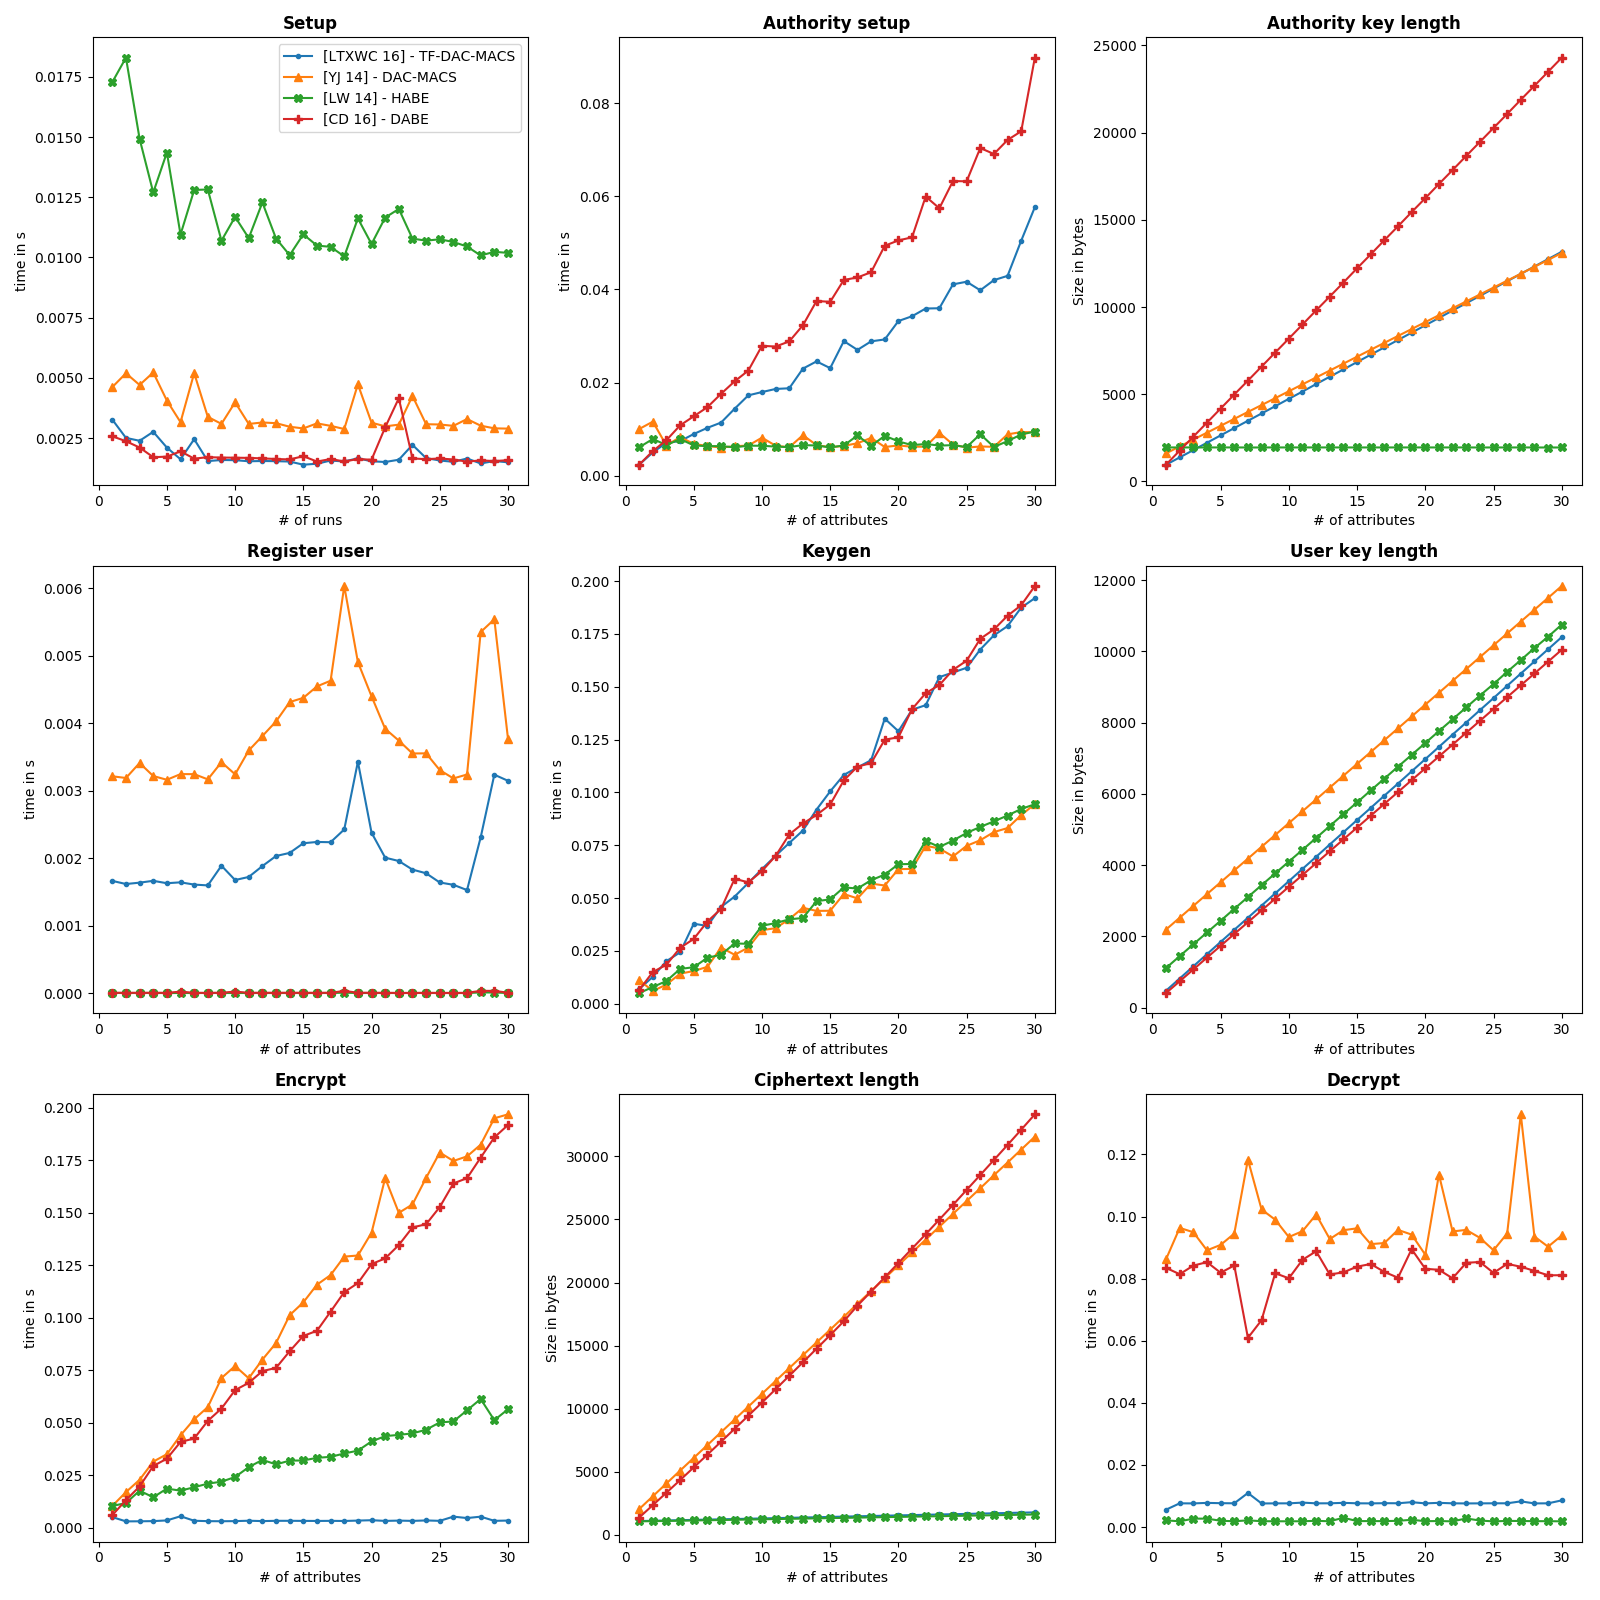
\includegraphics[width=1\linewidth]{img/maabe_comparisons.png}
    \caption{Performance and scalability comparison}
    \label{fig:maabe_comparison}
\end{figure*}

To compare the sub topics of \ac{MA-ABE} we need to extend the charm framework with an implementation of \ac{DABE}, \ac{HABE} and \ac{TF-DAC-MACS}. \ac{DAC-MACS} on the other hand exisited in the farmework already. 

In general we extracted five steps that each \ac{MA-ABE} scheme need to provide in some form. 
\begin{enumerate}
	\item \textbf{Setup:} The global setup phase where public paramter are settled.
	\item \textbf{Authority Setup:} \ac{AA}s can register themself to the central authority (if any) and compute their secret keys. Usally, the attribute secret keys are generated as well. 
	\item \textbf{Register User:} In the \ac{DAC-MACS} schemes user receive public and private key components. They are used for proxy decryption so that the server can help the user on decryption without revealing the plaintext. To do so the server generates a \textit{decryption token} which is encrypted with the users public key. Other schemes just assign the user a \ac{GID}. 
	\item \textbf{Kegen:} Attributes are assigned to user and the respective secret keys are generated.
	\item \textbf{Encrypt:} The cipher text is encrypted by the data owner under an access policy.
	\item \textbf{Decrypt:} The user (with the help of the server) decrypts the cipher text and revocers the secret message m. 
\end{enumerate}

This steps are shown and compared in \ref{fig:maabe_comparison}. As it turns out no scheme can be defined as the most performant or most scalabe one. All schemes performace roughly equally good. Some could argue that \ac{DAC-MACS} performed the worst, then \ac{DABE}, then \ac{TF-DAC-MACS} and the best performance has \ac{HABE}. 

However, for pratical usage especially the encryption and decryption performance is cural. There only \ac{TF-DAC-MACS} has an constant overhead while all other schemes are linear. If we further have a look at the table of requirements \ref{tab:ma_abe_comparisons}, we see that only two schemes satisfy all of the requirements: \ac{TF-DAC-MACS} and \ac{DABE}. \ac{DABE} profits also from the fact that it has a more fine grant access control then \ac{TF-DAC-MACS}. However, its revocation scheme is the disadventage that leave us with \ac{TF-DAC-MACS} as our final candidate. As mentioned in section \ref{sec:DABE} the implemented scheme uses indirct time-based revocation, which forces data owner to periodically reencrypt and reupload thier content. This is in a cloud storage system not really applicable. 

The comparison of \ac{TF-DAC-MACS} with other schemes of the \ac{DAC-MACS} family was left out in this work, since it was already done in the \ac{TF-DAC-MACS} paper \cite{li2017two}. Here some could easly see that \ac{TF-DAC-MACS} is currently the most performant scheme in the \ac{DAC-MACS} family.  